% SBiND 2027 (ICASSP 2027 satellite workshop) -- ICASSP style (spconf.sty)
% Build: pdflatex + bibtex + pdflatex x2.  tables/*.tex and numbers.tex are generated by src/make_paper_tables.py
\documentclass{article}
\usepackage{spconf,amsmath,amssymb,graphicx,booktabs,url}
\usepackage[font=small,labelfont=bf,skip=3pt]{caption}
\graphicspath{{../results/analysis/figures/}}
\newcommand{\nHC}{51}
\newcommand{\nND}{53}
\newcommand{\nD}{49}
\newcommand{\nFeat}{39}
\newcommand{\topAUC}{0.70}
\newcommand{\topLo}{0.59}
\newcommand{\topHi}{0.80}
\newcommand{\topQ}{0.019}
\newcommand{\topAdj}{0.71}
\newcommand{\topQadj}{0.009}
\newcommand{\topMedHC}{1.05}
\newcommand{\topMedND}{1.83}
\newcommand{\topMedD}{2.66}
\newcommand{\nSigRaw}{1}
\newcommand{\nSigAdj}{2}
\newcommand{\ddkFAUC}{0.66}
\newcommand{\ddkFLo}{0.54}
\newcommand{\ddkFHi}{0.77}
\newcommand{\ddkFAdj}{0.68}
\newcommand{\ddkFQadj}{0.026}
\newcommand{\ddkFQ}{0.110}
\newcommand{\ddkFDAUC}{0.86}
\newcommand{\ddkFDLo}{0.78}
\newcommand{\ddkFDHi}{0.93}
\newcommand{\jitPAUC}{0.61}
\newcommand{\jitPLo}{0.50}
\newcommand{\jitPHi}{0.72}
\newcommand{\jitPAdj}{0.63}
\newcommand{\jitPQadj}{0.153}
\newcommand{\jitPQ}{0.279}
\newcommand{\jitPDAUC}{0.65}
\newcommand{\jitPDLo}{0.53}
\newcommand{\jitPDHi}{0.76}
\newcommand{\vbreakAUC}{0.61}
\newcommand{\vbreakLo}{0.50}
\newcommand{\vbreakHi}{0.72}
\newcommand{\vbreakAdj}{0.63}
\newcommand{\vbreakQadj}{0.153}
\newcommand{\vbreakQ}{0.279}
\newcommand{\vbreakDAUC}{0.67}
\newcommand{\vbreakDLo}{0.55}
\newcommand{\vbreakDHi}{0.77}
\newcommand{\ddkrateAUC}{0.46}
\newcommand{\ddkrateLo}{0.35}
\newcommand{\ddkrateHi}{0.58}
\newcommand{\ddkrateAdj}{0.46}
\newcommand{\ddkrateQadj}{0.655}
\newcommand{\ddkrateQ}{0.733}
\newcommand{\ddkrateDAUC}{0.25}
\newcommand{\ddkrateDLo}{0.15}
\newcommand{\ddkrateDHi}{0.35}
\newcommand{\ioicvAUC}{0.54}
\newcommand{\ioicvLo}{0.43}
\newcommand{\ioicvHi}{0.66}
\newcommand{\ioicvAdj}{0.54}
\newcommand{\ioicvQadj}{0.623}
\newcommand{\ioicvQ}{0.733}
\newcommand{\ioicvDAUC}{0.59}
\newcommand{\ioicvDLo}{0.47}
\newcommand{\ioicvDHi}{0.71}
\newcommand{\vsaAUC}{0.43}
\newcommand{\vsaLo}{0.33}
\newcommand{\vsaHi}{0.55}
\newcommand{\vsaAdj}{0.41}
\newcommand{\vsaQadj}{0.342}
\newcommand{\vsaQ}{0.632}
\newcommand{\vsaDAUC}{0.30}
\newcommand{\vsaDLo}{0.20}
\newcommand{\vsaDHi}{0.41}
\newcommand{\fcrAUC}{0.59}
\newcommand{\fcrLo}{0.49}
\newcommand{\fcrHi}{0.70}
\newcommand{\fcrAdj}{0.59}
\newcommand{\fcrQadj}{0.316}
\newcommand{\fcrQ}{0.340}
\newcommand{\fcrDAUC}{0.74}
\newcommand{\fcrDLo}{0.64}
\newcommand{\fcrDHi}{0.84}
\newcommand{\sylrunAUC}{0.51}
\newcommand{\sylrunLo}{0.40}
\newcommand{\sylrunHi}{0.62}
\newcommand{\sylrunAdj}{0.49}
\newcommand{\sylrunQadj}{0.955}
\newcommand{\sylrunQ}{0.946}
\newcommand{\sylrunDAUC}{0.22}
\newcommand{\sylrunDLo}{0.13}
\newcommand{\sylrunDHi}{0.32}
\newcommand{\mptAUC}{0.49}
\newcommand{\mptLo}{0.38}
\newcommand{\mptHi}{0.61}
\newcommand{\mptAdj}{0.47}
\newcommand{\mptQadj}{0.820}
\newcommand{\mptQ}{0.977}
\newcommand{\mptDAUC}{0.26}
\newcommand{\mptDLo}{0.17}
\newcommand{\mptDHi}{0.36}
\newcommand{\intslopeAUC}{0.52}
\newcommand{\intslopeLo}{0.40}
\newcommand{\intslopeHi}{0.62}
\newcommand{\intslopeAdj}{0.50}
\newcommand{\intslopeQadj}{0.978}
\newcommand{\intslopeQ}{0.917}
\newcommand{\intslopeDAUC}{0.24}
\newcommand{\intslopeDLo}{0.15}
\newcommand{\intslopeDHi}{0.34}
\newcommand{\vowFAUC}{0.59}
\newcommand{\vowFLo}{0.47}
\newcommand{\vowFHi}{0.70}
\newcommand{\vowFAdj}{0.61}
\newcommand{\vowFQadj}{0.190}
\newcommand{\vowFQ}{0.340}
\newcommand{\vowFDAUC}{0.71}
\newcommand{\vowFDLo}{0.61}
\newcommand{\vowFDHi}{0.81}
\newcommand{\hnrAUC}{0.43}
\newcommand{\hnrLo}{0.31}
\newcommand{\hnrHi}{0.54}
\newcommand{\hnrAdj}{0.41}
\newcommand{\hnrQadj}{0.342}
\newcommand{\hnrQ}{0.548}
\newcommand{\hnrDAUC}{0.40}
\newcommand{\hnrDLo}{0.29}
\newcommand{\hnrDHi}{0.52}
\newcommand{\cppsAUC}{0.46}
\newcommand{\cppsLo}{0.35}
\newcommand{\cppsHi}{0.58}
\newcommand{\cppsAdj}{0.45}
\newcommand{\cppsQadj}{0.601}
\newcommand{\cppsQ}{0.733}
\newcommand{\cppsDAUC}{0.40}
\newcommand{\cppsDLo}{0.29}
\newcommand{\cppsDHi}{0.51}
\newcommand{\tkaAUC}{0.68}
\newcommand{\tkaLo}{0.57}
\newcommand{\tkaHi}{0.78}
\newcommand{\tkaBrier}{0.23}
\newcommand{\tkaDAUC}{0.86}
\newcommand{\tkaDLo}{0.77}
\newcommand{\tkaDHi}{0.93}
\newcommand{\mkaAUC}{0.47}
\newcommand{\mkaLo}{0.37}
\newcommand{\mkaHi}{0.59}
\newcommand{\mkaDAUC}{0.72}
\newcommand{\mkaDLo}{0.60}
\newcommand{\mkaDHi}{0.82}
\newcommand{\tpaAUC}{0.61}
\newcommand{\tpaLo}{0.49}
\newcommand{\tpaHi}{0.72}
\newcommand{\tpaBrier}{0.25}
\newcommand{\tpaDAUC}{0.87}
\newcommand{\tpaDLo}{0.80}
\newcommand{\tpaDHi}{0.94}
\newcommand{\mpaAUC}{0.49}
\newcommand{\mpaLo}{0.37}
\newcommand{\mpaHi}{0.60}
\newcommand{\mpaDAUC}{0.73}
\newcommand{\mpaDLo}{0.63}
\newcommand{\mpaDHi}{0.83}
\newcommand{\ttaAUC}{0.55}
\newcommand{\ttaLo}{0.44}
\newcommand{\ttaHi}{0.67}
\newcommand{\ttaBrier}{0.26}
\newcommand{\ttaDAUC}{0.80}
\newcommand{\ttaDLo}{0.70}
\newcommand{\ttaDHi}{0.89}
\newcommand{\mtaAUC}{0.39}
\newcommand{\mtaLo}{0.28}
\newcommand{\mtaHi}{0.49}
\newcommand{\mtaDAUC}{0.75}
\newcommand{\mtaDLo}{0.65}
\newcommand{\mtaDHi}{0.84}
\newcommand{\taAUC}{0.58}
\newcommand{\taLo}{0.46}
\newcommand{\taHi}{0.69}
\newcommand{\taBrier}{0.26}
\newcommand{\taDAUC}{0.73}
\newcommand{\taDLo}{0.63}
\newcommand{\taDHi}{0.83}
\newcommand{\maAUC}{0.44}
\newcommand{\maLo}{0.33}
\newcommand{\maHi}{0.55}
\newcommand{\maDAUC}{0.66}
\newcommand{\maDLo}{0.54}
\newcommand{\maDHi}{0.75}
\newcommand{\tiAUC}{0.59}
\newcommand{\tiLo}{0.48}
\newcommand{\tiHi}{0.70}
\newcommand{\tiBrier}{0.25}
\newcommand{\tiDAUC}{0.70}
\newcommand{\tiDLo}{0.59}
\newcommand{\tiDHi}{0.79}
\newcommand{\miAUC}{0.55}
\newcommand{\miLo}{0.45}
\newcommand{\miHi}{0.65}
\newcommand{\miDAUC}{0.78}
\newcommand{\miDLo}{0.69}
\newcommand{\miDHi}{0.87}
\newcommand{\toAUC}{0.48}
\newcommand{\toLo}{0.36}
\newcommand{\toHi}{0.60}
\newcommand{\toBrier}{0.27}
\newcommand{\toDAUC}{0.74}
\newcommand{\toDLo}{0.64}
\newcommand{\toDHi}{0.83}
\newcommand{\moAUC}{0.50}
\newcommand{\moLo}{0.38}
\newcommand{\moHi}{0.61}
\newcommand{\moDAUC}{0.63}
\newcommand{\moDLo}{0.52}
\newcommand{\moDHi}{0.75}
\newcommand{\tuAUC}{0.50}
\newcommand{\tuLo}{0.39}
\newcommand{\tuHi}{0.60}
\newcommand{\tuBrier}{0.28}
\newcommand{\tuDAUC}{0.79}
\newcommand{\tuDLo}{0.70}
\newcommand{\tuDHi}{0.88}
\newcommand{\muAUC}{0.54}
\newcommand{\muLo}{0.43}
\newcommand{\muHi}{0.64}
\newcommand{\muDAUC}{0.72}
\newcommand{\muDLo}{0.62}
\newcommand{\muDHi}{0.81}
\newcommand{\tvowAUC}{0.57}
\newcommand{\tvowLo}{0.45}
\newcommand{\tvowHi}{0.68}
\newcommand{\tvowBrier}{0.27}
\newcommand{\tvowDAUC}{0.81}
\newcommand{\tvowDLo}{0.73}
\newcommand{\tvowDHi}{0.89}
\newcommand{\mvowAUC}{0.56}
\newcommand{\mvowLo}{0.45}
\newcommand{\mvowHi}{0.67}
\newcommand{\mvowDAUC}{0.78}
\newcommand{\mvowDLo}{0.69}
\newcommand{\mvowDHi}{0.86}
\newcommand{\tddkAUC}{0.63}
\newcommand{\tddkLo}{0.52}
\newcommand{\tddkHi}{0.73}
\newcommand{\tddkBrier}{0.24}
\newcommand{\tddkDAUC}{0.85}
\newcommand{\tddkDLo}{0.77}
\newcommand{\tddkDHi}{0.93}
\newcommand{\mddkAUC}{0.41}
\newcommand{\mddkLo}{0.31}
\newcommand{\mddkHi}{0.52}
\newcommand{\mddkDAUC}{0.72}
\newcommand{\mddkDLo}{0.61}
\newcommand{\mddkDHi}{0.82}
\newcommand{\tallAUC}{0.58}
\newcommand{\tallLo}{0.48}
\newcommand{\tallHi}{0.69}
\newcommand{\tallBrier}{0.27}
\newcommand{\tallDAUC}{0.85}
\newcommand{\tallDLo}{0.76}
\newcommand{\tallDHi}{0.92}
\newcommand{\mallAUC}{0.50}
\newcommand{\mallLo}{0.38}
\newcommand{\mallHi}{0.61}
\newcommand{\mallDAUC}{0.77}
\newcommand{\mallDLo}{0.68}
\newcommand{\mallDHi}{0.86}
\newcommand{\tphonAUC}{0.64}
\newcommand{\tphonLo}{0.52}
\newcommand{\tphonHi}{0.74}
\newcommand{\tphonBrier}{0.24}
\newcommand{\tphonDAUC}{0.84}
\newcommand{\tphonDLo}{0.76}
\newcommand{\tphonDHi}{0.91}
\newcommand{\toneAUC}{0.66}
\newcommand{\toneLo}{0.56}
\newcommand{\toneHi}{0.77}
\newcommand{\toneBrier}{0.23}
\newcommand{\toneDAUC}{0.73}
\newcommand{\toneDLo}{0.63}
\newcommand{\toneDHi}{0.83}
\newcommand{\ttaoneAUC}{0.63}
\newcommand{\ttaoneLo}{0.52}
\newcommand{\ttaoneHi}{0.73}
\newcommand{\ttaoneBrier}{0.24}
\newcommand{\ttaoneDAUC}{0.63}
\newcommand{\ttaoneDLo}{0.51}
\newcommand{\ttaoneDHi}{0.73}
\newcommand{\tkaoneAUC}{0.65}
\newcommand{\tkaoneLo}{0.54}
\newcommand{\tkaoneHi}{0.75}
\newcommand{\tkaoneBrier}{0.24}
\newcommand{\tkaoneDAUC}{0.59}
\newcommand{\tkaoneDLo}{0.47}
\newcommand{\tkaoneDHi}{0.70}
\newcommand{\tddkoneAUC}{0.67}
\newcommand{\tddkoneLo}{0.57}
\newcommand{\tddkoneHi}{0.77}
\newcommand{\tddkoneBrier}{0.23}
\newcommand{\tddkoneDAUC}{0.72}
\newcommand{\tddkoneDLo}{0.61}
\newcommand{\tddkoneDHi}{0.82}
\newcommand{\mBestAUC}{0.57}
\newcommand{\nRep}{20}
\newcommand{\CVal}{0.3}
\newcommand{\fvcSylRho}{0.61}
\newcommand{\fvcSylQ}{0.000}
\newcommand{\fvcSylN}{101}
\newcommand{\mrcSylRho}{0.68}
\newcommand{\mrcSylQ}{0.000}
\newcommand{\mrcSylN}{101}
\newcommand{\bulSylRho}{0.67}
\newcommand{\bulSylQ}{0.000}
\newcommand{\bulSylN}{101}
\newcommand{\pumnsSylRho}{-0.39}
\newcommand{\pumnsSylQ}{0.002}
\newcommand{\pumnsSylN}{100}
\newcommand{\ndDyspVbRho}{-0.44}
\newcommand{\ndDyspVbQ}{0.039}
\newcommand{\ndDyspVbN}{53}
\newcommand{\ndDyspJitRho}{-0.35}
\newcommand{\ndDyspJitQ}{0.067}
\newcommand{\ndDyspJitN}{53}
\newcommand{\ndMrcSylRho}{0.39}
\newcommand{\ndMrcSylQ}{0.085}
\newcommand{\ndMrcSylN}{53}
\newcommand{\ndMrcIntRho}{0.36}
\newcommand{\ndMrcIntQ}{0.085}
\newcommand{\ndMrcIntN}{53}
\newcommand{\ndDurSylRho}{-0.43}
\newcommand{\ndDurSylQ}{0.053}
\newcommand{\ndDurSylN}{53}
\newcommand{\pumnsTremRho}{-0.30}
\newcommand{\pumnsTremQ}{0.021}
\newcommand{\pumnsTremN}{100}
\newcommand{\pumnsRateRho}{-0.33}
\newcommand{\pumnsRateQ}{0.014}
\newcommand{\pumnsRateN}{100}
\newcommand{\fvcFRho}{-0.33}
\newcommand{\fvcFQ}{0.003}
\newcommand{\fvcFN}{102}
\newcommand{\bulFRho}{-0.36}
\newcommand{\bulFQ}{0.001}
\newcommand{\bulFN}{102}
\newcommand{\ndallDyspRho}{-0.27}
\newcommand{\ndallDyspQ}{0.021}
\newcommand{\ndallDyspN}{97}
\newcommand{\eWanderAUC}{0.64}
\newcommand{\eWanderLo}{0.53}
\newcommand{\eWanderHi}{0.74}
\newcommand{\eWanderQ}{0.063}
\newcommand{\eWanderAdj}{0.66}
\newcommand{\eWanderQadj}{0.017}
\newcommand{\eWanderDAUC}{0.81}
\newcommand{\eWanderMedHC}{0.012}
\newcommand{\eWanderMedND}{0.024}
\newcommand{\eSlowAUC}{0.60}
\newcommand{\eSlowLo}{0.49}
\newcommand{\eSlowHi}{0.70}
\newcommand{\eSlowQ}{0.140}
\newcommand{\eSlowAdj}{0.62}
\newcommand{\eSlowQadj}{0.060}
\newcommand{\eSlowDAUC}{0.71}
\newcommand{\eSlowMedHC}{0.022}
\newcommand{\eSlowMedND}{0.036}
\newcommand{\eTremorAUC}{0.59}
\newcommand{\eTremorLo}{0.48}
\newcommand{\eTremorHi}{0.70}
\newcommand{\eTremorQ}{0.197}
\newcommand{\eTremorAdj}{0.61}
\newcommand{\eTremorQadj}{0.085}
\newcommand{\eTremorDAUC}{0.62}
\newcommand{\eTremorMedHC}{0.005}
\newcommand{\eTremorMedND}{0.008}
\newcommand{\eFlutterAUC}{0.63}
\newcommand{\eFlutterLo}{0.53}
\newcommand{\eFlutterHi}{0.73}
\newcommand{\eFlutterQ}{0.066}
\newcommand{\eFlutterAdj}{0.65}
\newcommand{\eFlutterQadj}{0.026}
\newcommand{\eFlutterDAUC}{0.75}
\newcommand{\eFlutterMedHC}{0.002}
\newcommand{\eFlutterMedND}{0.004}
\newcommand{\eWanderRelAUC}{0.55}
\newcommand{\eWanderRelLo}{0.44}
\newcommand{\eWanderRelHi}{0.67}
\newcommand{\eWanderRelQ}{0.495}
\newcommand{\eWanderRelAdj}{0.56}
\newcommand{\eWanderRelQadj}{0.464}
\newcommand{\eWanderRelDAUC}{0.69}
\newcommand{\eWanderRelMedHC}{0.286}
\newcommand{\eWanderRelMedND}{0.335}
\newcommand{\eTremorRelAUC}{0.49}
\newcommand{\eTremorRelLo}{0.38}
\newcommand{\eTremorRelHi}{0.60}
\newcommand{\eTremorRelQ}{0.895}
\newcommand{\eTremorRelAdj}{0.50}
\newcommand{\eTremorRelQadj}{0.990}
\newcommand{\eTremorRelDAUC}{0.33}
\newcommand{\eTremorRelMedHC}{0.120}
\newcommand{\eTremorRelMedND}{0.121}
\newcommand{\eFoldAUC}{0.66}
\newcommand{\eFoldLo}{0.56}
\newcommand{\eFoldHi}{0.76}
\newcommand{\eFoldQ}{0.029}
\newcommand{\eFoldAdj}{0.69}
\newcommand{\eFoldQadj}{0.009}
\newcommand{\eFoldDAUC}{0.81}
\newcommand{\eFoldMedHC}{0.499}
\newcommand{\eFoldMedND}{0.626}
\newcommand{\eOctVAUC}{0.58}
\newcommand{\eOctVLo}{0.47}
\newcommand{\eOctVHi}{0.69}
\newcommand{\eOctVQ}{0.247}
\newcommand{\eOctVAdj}{0.59}
\newcommand{\eOctVQadj}{0.176}
\newcommand{\eOctVDAUC}{0.68}
\newcommand{\eOctVMedHC}{0.015}
\newcommand{\eOctVMedND}{0.034}
\newcommand{\eMacroAUC}{0.66}
\newcommand{\eMacroLo}{0.55}
\newcommand{\eMacroHi}{0.76}
\newcommand{\eMacroQ}{0.029}
\newcommand{\eMacroAdj}{0.67}
\newcommand{\eMacroQadj}{0.016}
\newcommand{\eMacroDAUC}{0.72}
\newcommand{\eMacroMedHC}{0.732}
\newcommand{\eMacroMedND}{0.989}
\newcommand{\eMacroDetrAUC}{0.66}
\newcommand{\eMacroDetrLo}{0.55}
\newcommand{\eMacroDetrHi}{0.76}
\newcommand{\eMacroDetrQ}{0.029}
\newcommand{\eMacroDetrAdj}{0.67}
\newcommand{\eMacroDetrQadj}{0.016}
\newcommand{\eMacroDetrDAUC}{0.71}
\newcommand{\eMacroDetrMedHC}{0.599}
\newcommand{\eMacroDetrMedND}{0.813}
\newcommand{\eLagAUC}{0.48}
\newcommand{\eLagLo}{0.37}
\newcommand{\eLagHi}{0.59}
\newcommand{\eLagQ}{0.805}
\newcommand{\eLagAdj}{0.48}
\newcommand{\eLagQadj}{0.780}
\newcommand{\eLagDAUC}{0.40}
\newcommand{\eLagMedHC}{0.215}
\newcommand{\eLagMedND}{0.189}
\newcommand{\eMicroAUC}{0.54}
\newcommand{\eMicroLo}{0.43}
\newcommand{\eMicroHi}{0.65}
\newcommand{\eMicroQ}{0.687}
\newcommand{\eMicroAdj}{0.54}
\newcommand{\eMicroQadj}{0.567}
\newcommand{\eMicroDAUC}{0.51}
\newcommand{\eMicroMedHC}{0.468}
\newcommand{\eMicroMedND}{0.547}
\newcommand{\eOctDAUC}{0.70}
\newcommand{\eOctDLo}{0.59}
\newcommand{\eOctDHi}{0.80}
\newcommand{\eOctDQ}{0.009}
\newcommand{\eOctDAdj}{0.72}
\newcommand{\eOctDQadj}{0.002}
\newcommand{\eOctDDAUC}{0.71}
\newcommand{\eOctDMedHC}{0.004}
\newcommand{\eOctDMedND}{0.018}
\newcommand{\eOnsetAUC}{0.63}
\newcommand{\eOnsetLo}{0.52}
\newcommand{\eOnsetHi}{0.73}
\newcommand{\eOnsetQ}{0.066}
\newcommand{\eOnsetAdj}{0.63}
\newcommand{\eOnsetQadj}{0.047}
\newcommand{\eOnsetDAUC}{0.80}
\newcommand{\eOnsetMedHC}{1.254}
\newcommand{\eOnsetMedND}{1.547}
\newcommand{\eVotAUC}{0.65}
\newcommand{\eVotLo}{0.53}
\newcommand{\eVotHi}{0.76}
\newcommand{\eVotQ}{0.035}
\newcommand{\eVotAdj}{0.66}
\newcommand{\eVotQadj}{0.019}
\newcommand{\eVotDAUC}{0.72}
\newcommand{\eVotMedHC}{0.024}
\newcommand{\eVotMedND}{0.030}
\newcommand{\eRiseAUC}{0.54}
\newcommand{\eRiseLo}{0.43}
\newcommand{\eRiseHi}{0.66}
\newcommand{\eRiseQ}{0.687}
\newcommand{\eRiseAdj}{0.55}
\newcommand{\eRiseQadj}{0.503}
\newcommand{\eRiseDAUC}{0.76}
\newcommand{\eRiseMedHC}{0.070}
\newcommand{\eRiseMedND}{0.077}
\newcommand{\eRiseSdAUC}{0.53}
\newcommand{\eRiseSdLo}{0.41}
\newcommand{\eRiseSdHi}{0.64}
\newcommand{\eRiseSdQ}{0.727}
\newcommand{\eRiseSdAdj}{0.53}
\newcommand{\eRiseSdQadj}{0.725}
\newcommand{\eRiseSdDAUC}{0.65}
\newcommand{\eRiseSdMedHC}{0.136}
\newcommand{\eRiseSdMedND}{0.140}
\newcommand{\eIntWanderAUC}{0.63}
\newcommand{\eIntWanderLo}{0.52}
\newcommand{\eIntWanderHi}{0.73}
\newcommand{\eIntWanderQ}{0.069}
\newcommand{\eIntWanderAdj}{0.65}
\newcommand{\eIntWanderQadj}{0.026}
\newcommand{\eIntWanderDAUC}{0.80}
\newcommand{\eIntWanderMedHC}{0.455}
\newcommand{\eIntWanderMedND}{0.562}
\newcommand{\nExt}{22}
\newcommand{\nExtSigRaw}{5}
\newcommand{\nExtSigAdj}{9}
\newcommand{\pSylUmn}{-0.19}
\newcommand{\pSylUmnQ}{0.34}
\newcommand{\pSylLmn}{0.60}
\newcommand{\pSylLmnQ}{0.000}
\newcommand{\pMptUmn}{-0.04}
\newcommand{\pMptUmnQ}{0.78}
\newcommand{\pMptLmn}{0.49}
\newcommand{\pMptLmnQ}{0.000}
\newcommand{\pIntUmn}{-0.12}
\newcommand{\pIntUmnQ}{0.58}
\newcommand{\pIntLmn}{0.49}
\newcommand{\pIntLmnQ}{0.000}
\newcommand{\pRateUmn}{-0.19}
\newcommand{\pRateUmnQ}{0.34}
\newcommand{\pRateLmn}{0.35}
\newcommand{\pRateLmnQ}{0.002}
\newcommand{\pRiseUmn}{0.16}
\newcommand{\pRiseUmnQ}{0.36}
\newcommand{\pRiseLmn}{-0.48}
\newcommand{\pRiseLmnQ}{0.000}
\newcommand{\pFoldUmn}{-0.05}
\newcommand{\pFoldUmnQ}{0.77}
\newcommand{\pFoldLmn}{-0.31}
\newcommand{\pFoldLmnQ}{0.006}
\newcommand{\pTremUmn}{-0.25}
\newcommand{\pTremUmnQ}{0.26}
\newcommand{\pTremLmn}{-0.20}
\newcommand{\pTremLmnQ}{0.110}
\newcommand{\pSylFUmn}{-0.06}
\newcommand{\pSylFUmnQ}{0.77}
\newcommand{\pSylFLmn}{-0.10}
\newcommand{\pSylFLmnQ}{0.409}
\newcommand{\pUmnMinQ}{0.26}
\newcommand{\pUmnMaxAbs}{0.25}
\newcommand{\pNLmnSig}{17}
\newcommand{\pN}{61}
\newcommand{\gNdMinQ}{0.49}
\newcommand{\gNdAucLo}{0.33}
\newcommand{\gNdAucHi}{0.60}
\newcommand{\gNdNfast}{25}
\newcommand{\gNdN}{53}
\newcommand{\gIntRho}{-0.41}
\newcommand{\gIntQ}{0.000}
\newcommand{\gIntRhoDur}{-0.49}
\newcommand{\gIntAucFast}{0.30}
\newcommand{\gIntQFast}{0.019}
\newcommand{\gMptRho}{-0.28}
\newcommand{\gMptQ}{0.042}
\newcommand{\gMptRhoDur}{-0.43}
\newcommand{\gMptAucFast}{0.36}
\newcommand{\gMptQFast}{0.252}
\newcommand{\gFoldRho}{0.28}
\newcommand{\gFoldQ}{0.042}
\newcommand{\gFoldRhoDur}{0.33}
\newcommand{\gFoldAucFast}{0.59}
\newcommand{\gFoldQFast}{0.618}
\newcommand{\cPhonAUC}{0.64}
\newcommand{\cPhonLo}{0.53}
\newcommand{\cPhonHi}{0.74}
\newcommand{\cArtAUC}{0.54}
\newcommand{\cArtLo}{0.43}
\newcommand{\cArtHi}{0.65}
\newcommand{\cRespAUC}{0.40}
\newcommand{\cRespLo}{0.29}
\newcommand{\cRespHi}{0.52}
\newcommand{\dPhonArtDiff}{0.10}
\newcommand{\dPhonArtLo}{-0.01}
\newcommand{\dPhonArtHi}{0.21}
\newcommand{\dPhonArtP}{0.051}
\newcommand{\dPhonRespDiff}{0.24}
\newcommand{\dPhonRespLo}{0.09}
\newcommand{\dPhonRespHi}{0.38}
\newcommand{\dPhonRespP}{0.001}
\newcommand{\sPhonArtDiff}{0.09}
\newcommand{\sPhonArtLo}{-0.05}
\newcommand{\sPhonArtHi}{0.22}
\newcommand{\sPhonArtAUCtwo}{0.61}
\newcommand{\sPhonRespDiff}{0.18}
\newcommand{\sPhonRespLo}{0.05}
\newcommand{\sPhonRespHi}{0.29}
\newcommand{\sPhonRespAUCtwo}{0.53}
\newcommand{\sensAAUC}{0.70}
\newcommand{\sensAN}{53}
\newcommand{\sensALo}{0.59}
\newcommand{\sensAHi}{0.80}
\newcommand{\sensAP}{0.000}
\newcommand{\sensBAUC}{0.68}
\newcommand{\sensBN}{41}
\newcommand{\sensBLo}{0.57}
\newcommand{\sensBHi}{0.79}
\newcommand{\sensBP}{0.003}
\newcommand{\sensCAUC}{0.64}
\newcommand{\sensCN}{22}
\newcommand{\sensCLo}{0.50}
\newcommand{\sensCHi}{0.77}
\newcommand{\sensCP}{0.062}
\newcommand{\sensDAUC}{0.64}
\newcommand{\sensDN}{11}
\newcommand{\sensDLo}{0.45}
\newcommand{\sensDHi}{0.81}
\newcommand{\sensDP}{0.140}
\newcommand{\sensOctBAUC}{0.69}
\newcommand{\sensOctBLo}{0.58}
\newcommand{\sensOctBHi}{0.79}
\newcommand{\sensOctCAUC}{0.64}
\newcommand{\sensOctCLo}{0.51}
\newcommand{\sensOctCHi}{0.77}
\newcommand{\sensOctDAUC}{0.60}
\newcommand{\sensOctDLo}{0.41}
\newcommand{\sensOctDHi}{0.78}
\newcommand{\sensVowBAUC}{0.62}
\newcommand{\sensVowCAUC}{0.56}
\newcommand{\sensVowDAUC}{0.65}
\newcommand{\trkMin}{0.67}
\newcommand{\trkMax}{0.68}
\newcommand{\trkRhoMin}{0.82}
\newcommand{\trkRhoMax}{0.94}
\newcommand{\trkSameMin}{0.82}
\newcommand{\trkSameMax}{0.94}
\newcommand{\trkRpr}{0.61}
\newcommand{\trkRprP}{0.049}
\newcommand{\trkRprRho}{0.54}
\newcommand{\trkRprSame}{0.54}
\newcommand{\trkFoldMin}{0.63}
\newcommand{\trkFoldMax}{0.68}
\newcommand{\trkFoldRhoMin}{0.61}
\newcommand{\trkFoldRhoMax}{0.70}
\newcommand{\trkFoldSameMin}{0.92}
\newcommand{\trkFoldSameMax}{0.97}
\newcommand{\trkFoldRpr}{0.64}
\newcommand{\trkFoldRprP}{0.012}
\newcommand{\trkFoldRprRho}{0.58}
\newcommand{\trkFoldRprSame}{0.80}
\newcommand{\trkOctMin}{0.62}
\newcommand{\trkOctMax}{0.68}
\newcommand{\trkOctRhoMin}{0.65}
\newcommand{\trkOctRhoMax}{0.88}
\newcommand{\trkOctSameMin}{0.69}
\newcommand{\trkOctSameMax}{0.89}
\newcommand{\trkOctRpr}{0.59}
\newcommand{\trkOctRprP}{0.123}
\newcommand{\trkOctRprRho}{0.53}
\newcommand{\trkOctRprSame}{0.59}
\newcommand{\shrFlagged}{1033}
\newcommand{\shrGenuine}{663}
\newcommand{\shrGenuinePct}{64}
\newcommand{\shrFlagMed}{-3.5}
\newcommand{\shrCtrlMed}{-22.1}
\newcommand{\shrGenAUC}{0.69}
\newcommand{\shrGenP}{0.0008}
\newcommand{\shrSpurAUC}{0.64}
\newcommand{\shrSpurP}{0.008}
\newcommand{\octMedNDPct}{2.4}
\newcommand{\shrCtrlFP}{7}
\newcommand{\shrCtrlN}{3448}
\newcommand{\shrCtrlAbove}{238}
\newcommand{\shrDown}{807}
\newcommand{\shrUp}{226}
\newcommand{\shrDownGenuine}{502}
\newcommand{\shrDownPct}{62}
\newcommand{\shrDownMed}{-3.6}
\newcommand{\shrDownGenAUC}{0.66}
\newcommand{\shrDownGenP}{0.0029}
\newcommand{\shrDownSpurAUC}{0.65}
\newcommand{\shrUpAUC}{0.59}
\newcommand{\covAdjAUC}{0.75}
\newcommand{\covAdjP}{<10^{-4}}
\newcommand{\iccAll}{0.63}
\newcommand{\iccHC}{0.66}
\newcommand{\iccN}{144}
\newcommand{\shMin}{0.63}
\newcommand{\shMax}{0.77}
\newcommand{\sbMin}{0.77}
\newcommand{\sbMax}{0.87}
\newcommand{\btMin}{0.57}
\newcommand{\btMax}{0.65}
\newcommand{\covSnrAUC}{0.47}
\newcommand{\covSnrRhoHC}{-0.24}
\newcommand{\covSnrRho}{-0.17}
\newcommand{\covLevelAUC}{0.56}
\newcommand{\covLevelRhoHC}{-0.38}
\newcommand{\covLevelRho}{-0.22}
\newcommand{\covRateAUC}{0.46}
\newcommand{\covRateRhoHC}{0.40}
\newcommand{\covRateRho}{0.23}
\newcommand{\covNsylAUC}{0.52}
\newcommand{\covNsylRhoHC}{0.15}
\newcommand{\covNsylRho}{0.03}
\newcommand{\covFAUC}{0.48}
\newcommand{\covFRhoHC}{-0.16}
\newcommand{\covFRho}{-0.16}
\newcommand{\gAllAUC}{0.67}
\newcommand{\gAllLo}{0.56}
\newcommand{\gAllHi}{0.78}
\newcommand{\gAllN}{24}
\newcommand{\gIAUC}{0.73}
\newcommand{\gILo}{0.62}
\newcommand{\gIHi}{0.82}
\newcommand{\gIN}{12}
\newcommand{\gAAUC}{0.66}
\newcommand{\gALo}{0.55}
\newcommand{\gAHi}{0.77}
\newcommand{\gAN}{12}
\newcommand{\gPaAUC}{0.64}
\newcommand{\gPaLo}{0.53}
\newcommand{\gPaHi}{0.75}
\newcommand{\gPaN}{12}
\newcommand{\gKaAUC}{0.66}
\newcommand{\gKaLo}{0.56}
\newcommand{\gKaHi}{0.77}
\newcommand{\gKaN}{12}
\newcommand{\gAllMAUC}{0.55}
\newcommand{\gAllMLo}{0.44}
\newcommand{\gAllMHi}{0.66}
\newcommand{\gAllMN}{102}
\newcommand{\gIMAUC}{0.65}
\newcommand{\gIMLo}{0.55}
\newcommand{\gIMHi}{0.76}
\newcommand{\gIMN}{51}
\newcommand{\gBestTask}{/i/}
\newcommand{\gBestAUC}{0.73}
\newcommand{\gSingleMin}{0.60}
\newcommand{\gSingleMax}{0.73}
\newcommand{\gWorstTask}{/ta/}
\newcommand{\relPaAUC}{0.67}
\newcommand{\relPaP}{0.003}
\newcommand{\relTaAUC}{0.56}
\newcommand{\relTaP}{0.276}
\newcommand{\relKaAUC}{0.63}
\newcommand{\relKaP}{0.026}
\newcommand{\rSubhAUC}{0.64}
\newcommand{\rSubhLo}{0.53}
\newcommand{\rSubhHi}{0.74}
\newcommand{\rSubhP}{0.016}
\newcommand{\rSubhMedHC}{2.5}
\newcommand{\rSubhMedND}{7.4}
\newcommand{\rSubhRprAUC}{0.58}
\newcommand{\rSubhRprLo}{0.46}
\newcommand{\rSubhRprHi}{0.68}
\newcommand{\rSubhRprP}{0.168}
\newcommand{\rSubhRprMedHC}{5.2}
\newcommand{\rSubhRprMedND}{9.1}
\newcommand{\rSubhMedAUC}{0.61}
\newcommand{\rSubhMedLo}{0.50}
\newcommand{\rSubhMedHi}{0.72}
\newcommand{\rSubhMedP}{0.052}
\newcommand{\rSubhMedMedHC}{18.9}
\newcommand{\rSubhMedMedND}{28.9}
\newcommand{\rUnflAUC}{0.62}
\newcommand{\rUnflLo}{0.51}
\newcommand{\rUnflHi}{0.72}
\newcommand{\rUnflP}{0.037}
\newcommand{\rUnflMedHC}{1.3}
\newcommand{\rUnflMedND}{4.0}
\newcommand{\rOctAUC}{0.70}
\newcommand{\rOctLo}{0.60}
\newcommand{\rOctHi}{0.79}
\newcommand{\rOctP}{<0.001}
\newcommand{\rOctMedHC}{0.5}
\newcommand{\rOctMedND}{2.4}
\newcommand{\rOctTrimAUC}{0.70}
\newcommand{\rOctTrimLo}{0.60}
\newcommand{\rOctTrimHi}{0.80}
\newcommand{\rOctTrimP}{<0.001}
\newcommand{\rOctTrimMedHC}{0.0}
\newcommand{\rOctTrimMedND}{1.9}
\newcommand{\rOctEarlyAUC}{0.70}
\newcommand{\rOctEarlyLo}{0.60}
\newcommand{\rOctEarlyHi}{0.79}
\newcommand{\rOctEarlyP}{<0.001}
\newcommand{\rOctEarlyMedHC}{0.0}
\newcommand{\rOctEarlyMedND}{1.6}
\newcommand{\rOctLateAUC}{0.67}
\newcommand{\rOctLateLo}{0.56}
\newcommand{\rOctLateHi}{0.76}
\newcommand{\rOctLateP}{0.003}
\newcommand{\rOctLateMedHC}{0.0}
\newcommand{\rOctLateMedND}{3.2}
\newcommand{\rSdAUC}{0.70}
\newcommand{\rSdLo}{0.60}
\newcommand{\rSdHi}{0.80}
\newcommand{\rSdP}{<0.001}
\newcommand{\rFoldAUC}{0.66}
\newcommand{\rFoldLo}{0.54}
\newcommand{\rFoldHi}{0.76}
\newcommand{\rFoldP}{0.006}
\newcommand{\rSdTrimAUC}{0.69}
\newcommand{\rSdTrimLo}{0.58}
\newcommand{\rSdTrimHi}{0.79}
\newcommand{\rSdTrimP}{<0.001}
\newcommand{\rFoldTrimAUC}{0.65}
\newcommand{\rFoldTrimLo}{0.53}
\newcommand{\rFoldTrimHi}{0.75}
\newcommand{\rFoldTrimP}{0.011}
\newcommand{\rPosHCLast}{63}
\newcommand{\rPosHCLastThree}{31}
\newcommand{\rUnflRateHC}{5.9}
\newcommand{\rPosHCN}{142}
\newcommand{\rPosNDLast}{41}
\newcommand{\rPosNDLastThree}{12}
\newcommand{\rUnflRateND}{7.9}
\newcommand{\rPosNDN}{545}
\newcommand{\rSingleRun}{92}
\newcommand{\rNucLastThree}{6}
\newcommand{\rDropLast}{3}
\newcommand{\idvIntVAUC}{0.61}
\newcommand{\idvIntVP}{0.051}
\newcommand{\idvIntVMedHC}{66.9}
\newcommand{\idvIntVMedND}{68.4}
\newcommand{\idvVoicedDAUC}{0.40}
\newcommand{\idvVoicedDP}{0.095}
\newcommand{\idvVoicedDMedHC}{0.5}
\newcommand{\idvVoicedDMedND}{0.4}
\newcommand{\idvDurVAUC}{0.49}
\newcommand{\idvDurVP}{0.899}
\newcommand{\idvDurVMedHC}{16.0}
\newcommand{\idvDurVMedND}{14.7}
\newcommand{\idvDurDAUC}{0.55}
\newcommand{\idvDurDP}{0.407}
\newcommand{\idvDurDMedHC}{18.0}
\newcommand{\idvDurDMedND}{18.3}
\newcommand{\idvIntDAUC}{0.49}
\newcommand{\idvIntDP}{0.884}
\newcommand{\idvIntDMedHC}{59.4}
\newcommand{\idvIntDMedND}{58.6}
\newcommand{\idvBlock}{0.64}
\newcommand{\idvNoInt}{0.52}
\newcommand{\idvNoVoiced}{0.56}
\newcommand{\idvNoDur}{0.65}
\newcommand{\trkRprQ}{0.28}
\newcommand{\trkFoldRprQ}{0.24}
\newcommand{\trkFoldCcQ}{0.13}
\newcommand{\trkOctRprQ}{0.38}
\newcommand{\abFloorAUC}{0.47}
\newcommand{\abFloorLo}{0.35}
\newcommand{\abFloorHi}{0.57}
\newcommand{\abFzDdkMin}{0.64}
\newcommand{\abFzDdkMax}{0.69}
\newcommand{\abFzVowMin}{0.42}
\newcommand{\abFzVowMax}{0.60}
\newcommand{\abVqDdkMin}{0.50}
\newcommand{\abVqDdkMax}{0.52}
\newcommand{\abVqVowMin}{0.53}
\newcommand{\abVqVowMax}{0.67}
\newcommand{\abIdvDdkMin}{0.51}
\newcommand{\abIdvDdkMax}{0.57}
\newcommand{\abIdvVowMin}{0.56}
\newcommand{\abIdvVowMax}{0.61}
\newcommand{\abNfDdkMin}{0.50}
\newcommand{\abNfDdkMax}{0.57}
\newcommand{\abNfVowMin}{0.63}
\newcommand{\abNfVowMax}{0.74}
\newcommand{\abAllDdkMin}{0.60}
\newcommand{\abAllDdkMax}{0.66}
\newcommand{\abAllVowMin}{0.63}
\newcommand{\abAllVowMax}{0.73}
\newcommand{\abFzMed}{0.58}
\newcommand{\abFzMin}{0.42}
\newcommand{\abFzMax}{0.69}
\newcommand{\abFzAll}{0.68}
\newcommand{\abFzAllLo}{0.57}
\newcommand{\abFzAllHi}{0.78}
\newcommand{\abFzPa}{0.69}
\newcommand{\abFzTa}{0.64}
\newcommand{\abFzKa}{0.65}
\newcommand{\abFzI}{0.56}
\newcommand{\abFzA}{0.60}
\newcommand{\abFzE}{0.42}
\newcommand{\abVqMed}{0.53}
\newcommand{\abVqMin}{0.50}
\newcommand{\abVqMax}{0.67}
\newcommand{\abVqAll}{0.57}
\newcommand{\abVqAllLo}{0.45}
\newcommand{\abVqAllHi}{0.68}
\newcommand{\abVqPa}{0.51}
\newcommand{\abVqTa}{0.50}
\newcommand{\abVqKa}{0.52}
\newcommand{\abVqI}{0.67}
\newcommand{\abVqA}{0.53}
\newcommand{\abVqE}{0.60}
\newcommand{\abIdvMed}{0.58}
\newcommand{\abIdvMin}{0.51}
\newcommand{\abIdvMax}{0.61}
\newcommand{\abIdvAll}{0.64}
\newcommand{\abIdvAllLo}{0.53}
\newcommand{\abIdvAllHi}{0.75}
\newcommand{\abIdvPa}{0.55}
\newcommand{\abIdvTa}{0.51}
\newcommand{\abIdvKa}{0.57}
\newcommand{\abIdvI}{0.61}
\newcommand{\abIdvA}{0.60}
\newcommand{\abIdvE}{0.59}
\newcommand{\abNfMed}{0.64}
\newcommand{\abNfMin}{0.50}
\newcommand{\abNfMax}{0.74}
\newcommand{\abNfAll}{0.67}
\newcommand{\abNfAllLo}{0.56}
\newcommand{\abNfAllHi}{0.77}
\newcommand{\abNfPa}{0.54}
\newcommand{\abNfTa}{0.50}
\newcommand{\abNfKa}{0.57}
\newcommand{\abNfI}{0.74}
\newcommand{\abNfA}{0.65}
\newcommand{\abNfE}{0.70}
\newcommand{\abAllMed}{0.66}
\newcommand{\abAllMin}{0.60}
\newcommand{\abAllMax}{0.73}
\newcommand{\abAllAll}{0.67}
\newcommand{\abAllAllLo}{0.57}
\newcommand{\abAllAllHi}{0.78}
\newcommand{\abAllPa}{0.64}
\newcommand{\abAllTa}{0.60}
\newcommand{\abAllKa}{0.66}
\newcommand{\abAllI}{0.73}
\newcommand{\abAllA}{0.66}
\newcommand{\abAllE}{0.68}
\newcommand{\permPhonObs}{0.64}
\newcommand{\permPhonNull}{0.50}
\newcommand{\permPhonLo}{0.35}
\newcommand{\permPhonHi}{0.63}
\newcommand{\permPhonP}{0.025}
\newcommand{\permPhonExcess}{0.14}
\newcommand{\permArtObs}{0.54}
\newcommand{\permArtNull}{0.51}
\newcommand{\permArtLo}{0.36}
\newcommand{\permArtHi}{0.64}
\newcommand{\permArtP}{0.353}
\newcommand{\permArtExcess}{0.03}
\newcommand{\permRespObs}{0.40}
\newcommand{\permRespNull}{0.50}
\newcommand{\permRespLo}{0.35}
\newcommand{\permRespHi}{0.64}
\newcommand{\permRespP}{0.881}
\newcommand{\permRespExcess}{-0.10}
\newcommand{\permGenObs}{0.67}
\newcommand{\permGenNull}{0.49}
\newcommand{\permGenLo}{0.32}
\newcommand{\permGenHi}{0.62}
\newcommand{\permGenP}{0.010}
\newcommand{\permGenExcess}{0.18}
\newcommand{\permFloorObs}{0.47}
\newcommand{\permFloorNull}{0.48}
\newcommand{\permFloorLo}{0.28}
\newcommand{\permFloorHi}{0.63}
\newcommand{\permFloorP}{0.567}
\newcommand{\permFloorExcess}{-0.01}
\newcommand{\permN}{200}
\newcommand{\cHCN}{51}
\newcommand{\cHCAge}{63.0}
\newcommand{\cHCAgeSD}{10.4}
\newcommand{\cHCMale}{63}
\newcommand{\cNDN}{53}
\newcommand{\cNDAge}{60.7}
\newcommand{\cNDAgeSD}{11.2}
\newcommand{\cNDMale}{62}
\newcommand{\cNDBulb}{0}
\newcommand{\cNDSpin}{53}
\newcommand{\cNDFrs}{39}
\newcommand{\cNDFrsQa}{31}
\newcommand{\cNDFrsQb}{43}
\newcommand{\cNDFvc}{92}
\newcommand{\cDN}{49}
\newcommand{\cDAge}{65.0}
\newcommand{\cDAgeSD}{12.6}
\newcommand{\cDMale}{65}
\newcommand{\cDBulb}{20}
\newcommand{\cDSpin}{29}
\newcommand{\cDFrs}{33}
\newcommand{\cDFrsQa}{27}
\newcommand{\cDFrsQb}{39}
\newcommand{\cDFvc}{74}

\ninept
\raggedbottom

\title{Which speech measures differ when ALS speech is rated normal?\\ Between-syllable laryngeal instability}
\twoauthors{Allan Bola\~nos\thanks{Code, extracted features and supplementary tables: \texttt{github.com/AllanDBB/sbind-als}.}}
  {Escuela de Ingenier\'ia en Computaci\'on\\ Instituto Tecnol\'ogico de Costa Rica\\ \texttt{adbyb.es@gmail.com}}
  {Nicol\'as Florez}
  {Escuela de Ingenier\'ia en Computadores\\ Instituto Tecnol\'ogico de Costa Rica\\ \texttt{florezjnicolas@gmail.com}}

\begin{document}
\maketitle

\begin{abstract}
Speech in amyotrophic lateral sclerosis (ALS) is graded clinically with one perceptual item of the revised ALS Functional Rating Scale. On the public VOC-ALS database (\nHC{} controls, \nND{} patients with normal-rated speech, \nD{} with dysarthria) we ask which of \nFeat{} interpretable measures differ in the normal-rated group and what the difference consists of. Only one passes false-discovery control: the semitone spread of fundamental frequency ($F_0$) across the syllable nuclei of /pa/, /ta/, /ka/ repetitions (area under the receiver operating characteristic curve, AUC \topAUC). Articulatory and respiratory composites stay within their permutation nulls, although the phonatory--articulatory difference is uncertain (\dPhonArtDiff{} [$\dPhonArtLo$, \dPhonArtHi]). The spread lies between syllables, persists without the end of each breath run, and comes with more subharmonic re-onsets. Both depend on the pitch tracker: with an independent one the spread falls to \trkRpr{} ($p=\trkRprP$) and a spectral subharmonic share to \rSubhRprAUC, whereas the octave-folded spread is stable (\rFoldAUC{} vs.\ \trkFoldRpr) but only nominal.
\end{abstract}

\begin{keywords}
amyotrophic lateral sclerosis, bulbar dysfunction, speech biomarkers, laryngeal instability, subharmonics
\end{keywords}

\section{Introduction}
\label{sec:intro}
Amyotrophic lateral sclerosis (ALS) destroys upper and lower motor neurons. Bulbar involvement---weakness or spasticity of the face, tongue, larynx and pharynx---causes dysarthria and dysphagia, presents first in 20--30\% of patients, and is what patients report as most disabling~\cite{feldman2022als,tomik2010dysarthria}. Recognising it early matters because voice banking, augmentative communication and swallowing management work best when planned before function is lost~\cite{green2013bulbar}. Yet routine care grades speech with one perceptual item of the revised ALS Functional Rating Scale (ALSFRS-R)~\cite{cedarbaum1999alsfrsr}, scored 0--4 (4~=~normal) and insensitive to early change~\cite{green2013bulbar,allison2017diagnostic}.

That acoustic measures can differ before a listener hears a change is not new. Silbergleit et al.\ found altered frequency range and phonatory stability in sustained phonation of ALS patients with perceptually normal voice~\cite{silbergleit1997}; Stegmann et al.\ found lower speaking rate and articulatory precision, relative to healthy controls, in read sentences of patients whose ALSFRS-R speech, salivation and swallowing items were all normal, and tracked them remotely~\cite{stegmann2020early}. The paper releasing the Italian VOC-ALS database~\cite{dubbioso2024vocals} reported that the standard deviation (SD) of the fundamental frequency ($F_0$) of vowels and syllables, computed over each recording, identifies ALS and separates dysarthria classes, although in its five-class, Bonferroni-corrected comparisons the /pa/ value of controls differed from every class except the non-dysarthric one; later work frames the problem as detection or severity classification against the clinical rating~\cite{dubbioso2024precision,vashkevich2021,tena2021}. What remains open for a person whose speech is rated normal is \emph{which} measurable change is present, what the $F_0$ spread of a syllable train consists of at the signal level, how it relates to the motor pathway, and how far it can be trusted. We address this with the speech-subsystem view of bulbar ALS~\cite{rong2015subsystem,kent2003typology} and the validation standards proposed for digital biomarkers~\cite{goldsack2020v3,rusz2021biomarkers}. Contributions: (i) effect sizes for \nFeat{} interpretable measures in normal-rated speech, with false-discovery control, rank-based age/sex adjustment, chance references for every model (age/sex floor, permutation null, ablation of a generic descriptor set) and sensitivity tiers by bulbar findings; (ii) a signal-level decomposition of the syllable $F_0$ spread into between-/within-syllable, octave-level (subharmonic) and voice-onset components, with a spectral subharmonic measure free of per-nucleus octave decisions and the position of events within runs; (iii) sensitivity to the pitch tracker, including an independent one, and to recording covariates; (iv) clinical anchoring, including upper- vs.\ lower-motor-neuron proxies and progression.

\section{Data}
\label{sec:data}
VOC-ALS~\cite{dubbioso2024vocals} (Synapse \texttt{syn53009474}) has 153 Italian-speaking participants recruited consecutively at one ALS centre (Naples): 102 patients meeting the revised El Escorial criteria and 51 age- and sex-matched healthy controls (HC), each recorded once with a smartphone app (Samsung Galaxy S8+, 20\,cm, 8\,kHz, 16-bit) while sustaining /a/, /e/, /i/, /o/, /u/ for at least 5\,s and repeating /pa/, /ta/, /ka/ (diadochokinesis, DDK; self-paced, median 2.5 syllables/s). Patients were characterised with the ALSFRS-R and its items, forced vital capacity (FVC\,\%), Medical Research Council strength of head muscles (MRC, 0--15), the Penn Upper Motor Neuron Score bulbar sub-score (PUMNS, 0--4; one value of 7 treated as missing) and onset region. Three groups follow from the ALSFRS-R speech item: \textbf{HC} ($n=\cHCN$; age \cHCAge{} (SD \cHCAgeSD)); \textbf{ALS-ND}, normal-rated speech, item $=4$ ($n=\cNDN$; \cNDAge{} (\cNDAgeSD); all spinal onset; ALSFRS-R median \cNDFrs{} (IQR \cNDFrsQa--\cNDFrsQb)); \textbf{ALS-D}, dysarthria, item $<4$ ($n=\cDN$; \cDAge{} (\cDAgeSD); \cDBulb{} bulbar/\cDSpin{} spinal onset; ALSFRS-R \cDFrs{} (\cDFrsQa--\cDFrsQb); 31 mild, 13 moderate, 5 severe). As all ALS-ND patients have spinal onset, the primary contrast HC vs.\ ALS-ND asks whether speech differs in spinal-onset patients whom a neurologist rates as speaking normally; ALS-ND is 2.3 years younger than HC on average (adjusted below). ``Normal-rated'' describes the rating, not the bulbar examination: \sensBN{} of the \nND{} also have normal salivation and swallowing items, \sensCN{} full head-muscle strength as well, and \sensDN{} a PUMNS bulbar score of 0 in addition.

\begin{figure}[t]
\centering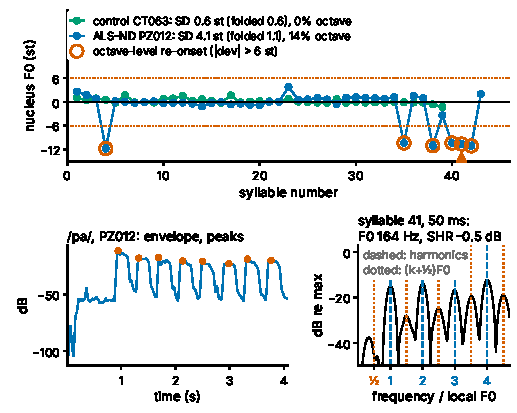
\includegraphics[width=\columnwidth]{fig0_example}
\caption{The marker on real data (/pa/, 8\,kHz smartphone audio). Top: median $F_0$ of each syllable nucleus in semitones re the speaker's median, for one control and one ALS-ND patient chosen as a clear example (ALS-ND median share of octave events, three syllable tasks: \rOctMedND\%); octave-level re-onsets circled. Bottom left: energy envelope with detected syllable peaks (first 8). Bottom right: 50\,ms spectrum of the arrowed nucleus, the clearest of those confirmed by the subharmonic-to-harmonic ratio (SHR) with subharmonics weaker than harmonics: peaks at $(k+\tfrac12)$ times the local $F_0$ mark subharmonic phonation (here period doubling) rather than a tracking error. Here the events cluster late in the run (see Sec.~\ref{sec:results}).}
\label{fig:example}
\end{figure}

\section{Methods}
\label{sec:methods}
\textbf{Signal processing and main measures (\nFeat).} All measures are computed with Praat 6.4~\cite{boersma2021praat} through Parselmouth~\cite{jadoul2018parselmouth}. The primary $F_0$ contour is Praat's cross-correlation tracker (\texttt{To Pitch (cc)}: floor 60\,Hz, ceiling 500\,Hz, 10\,ms step, other parameters at defaults); our jitter, shimmer, harmonics-to-noise ratio (HNR) and mean $F_0$ agree with the released values (Spearman $\rho$ 0.95--0.99). For each vowel the steady segment is the longest voiced run (gaps $\le$150\,ms bridged) minus 100\,ms at each end. In the DDK task, syllables are segmented from a 20\,ms RMS energy envelope (5\,ms hop, 30\,ms smoothing) by two-pass peak picking (peaks above $\max$(99th percentile $-$\,20\,dB, 5th percentile $+$\,6\,dB) with 4\,dB prominence, $\geq$90\,ms apart; the second pass imposes a spacing of 0.6 times the median interval of the first); the \emph{nucleus $F_0$} of a syllable is the median of the voiced frames within $\pm$40\,ms of its energy peak, and the SD across the sequence of its value in semitones (st) is the \emph{syllable $F_0$ SD} (Fig.~\ref{fig:example}). \emph{Phonation} (20): $F_0$ SD in st over the steady segment and over all voiced frames, drift and tremor indices, voice breaks, three jitter and four shimmer variants, HNR, smoothed cepstral peak prominence (CPPS)~\cite{maryn2010cpps}, spectral balance, intensity SD, syllable $F_0$ SD. \emph{Articulation} (12): median F1/F2 per vowel with vowel space area, formant centralisation ratio (FCR) and F2 /i/--/u/ ratio~\cite{sapir2010fcr}, F1/F2 instability, and DDK timing from the envelope peaks (rate, interval coefficient of variation (CV) and robust CV, slowing, amplitude variability, gap ratio, voiced fraction). \emph{Respiratory support} (7): longest phonation, voiced duration, intensity decline and drop, syllables per uninterrupted run (a new run starts after an interval longer than 2.5 times the median), pause fraction, amplitude decay. Vowel measures are averaged over vowels and DDK measures over syllable types. DDK measures needing five nuclei are missing for 1/53 ALS-ND and 4/49 ALS-D patients (median-imputed in models). Level and SNR are the 95th percentile of the envelope and its distance to the 5th percentile (dB).

\textbf{Time scale, voice re-initiation and subharmonics (\nExt{} exploratory measures).} A nucleus or frame deviating by more than 6\,st from its recording's median is an \emph{octave-level event}; spread measures below use the octave-folded contour (deviations folded by multiples of 12\,st), so that spread and octave events are separated. Vowels (10): the Welch modulation spectrum of the detrended st contour (100\,Hz, 4\,s segments, 50\% overlap) integrated over 0.25--1, 1--4, 4--8 and 8--15\,Hz, the 0.25--1 and 4--8\,Hz shares, the folded $F_0$ SD, the share of octave-level frames, and the 0.25--1 and 4--8\,Hz power of the intensity contour. DDK (5), from a 2\,ms pitch track (nuclei with $\geq$5 voiced frames): within-nucleus $F_0$ SD, across-syllable SD of nucleus medians, its detrended version, lag-1 autocorrelation, share of octave-level nuclei. Voice re-initiation (7, unfolded): mean absolute value and SD across syllables of the $F_0$ deviation in the first 30\,ms of voicing, and the SD of its slope; the burst-to-voicing delay (a voice onset time proxy: first voiced 2\,ms pitch frame minus the onset of the 2--3.9\,kHz burst envelope; task medians /pa/ $<$ /ta/ $<$ /ka/) and its SD; the 10--90\,\% amplitude rise time and its SD. \emph{Subharmonics}: a subharmonic-to-harmonic ratio (SHR) adapted from Sun~\cite{sun2002shr}: in a 50\,ms Hann window at the nucleus, the summed energy at odd multiples of a candidate fundamental relative to that at even multiples; SHR $> -6$\,dB counts as subharmonic phonation (period doubling, or a drop into a creak-like register). It is computed for the octave-down nuclei of the main 10\,ms track (candidate: the tracked value), for unflagged nuclei at half their $F_0$ (control), and, free of per-nucleus octave decisions, for \emph{every} nucleus at half its octave-folded $F_0$ (from Praat or REAPER) or at half the speaker's median, giving each speaker's share of subharmonic nuclei.

\textbf{Statistics and chance references.} For each measure and contrast: AUC (the probability that a patient's value exceeds a control's) with 95\% bootstrap CI (2000 resamples), Mann--Whitney $p$ corrected by Benjamini--Hochberg ($q$) within the \nFeat{} main or the \nExt{} exploratory measures, and an age- and sex-adjusted AUC from rank-based residuals (ranks of the measure regressed on ranks of age and sex). Composites are out-of-fold predictions of an $\ell_2$-logistic model on each subsystem's measures (imputation and standardisation fitted within training folds, $C=\CVal$, age and sex as covariates) under \nRep$\times$5-fold stratified cross-validation; the same model gives per-task AUCs. Cross-validated AUC varies widely under the null and can fall well below 0.5, so every composite is read against the same model with age and sex only and against a permutation null (labels shuffled \permN{} times, 3$\times$5-fold each), and composites are compared by a paired bootstrap of AUC differences. The generic reference set has 12 descriptors per task ($F_0$ mean, SD, 10--90 range and slope in st; jitter, shimmer, HNR; intensity mean, SD and range, voiced fraction, duration), with and without mel-frequency cepstral coefficient (MFCC) statistics, and is ablated by block. Robustness: the syllable $F_0$ SD recomputed with Praat's autocorrelation tracker, with a 75\,Hz floor, and with REAPER~\cite{talkin2015reaper}, an independent epoch-based tracker; the contrast repeated without the last \rDropLast{} syllables of each pause-delimited run; SNR, level, DDK rate, syllable count and mean $F_0$ compared between groups, the first four (with age and sex) removed by rank-based residualisation. Within-session consistency: intraclass correlation ICC(2,1) across /pa/, /ta/, /ka/ and split-half (odd vs.\ even syllables, Spearman--Brown); no test--retest data exist. Clinical anchoring: Spearman correlations within patients (Benjamini--Hochberg per score), partial correlations with PUMNS controlling MRC and age and vice versa (rank residuals), and the dataset's progression rate $(48-\mathrm{ALSFRS\text{-}R})/\mathrm{duration}$ (fast $\geq$0.5/month). Fixed seed throughout.

\section{Results}
\label{sec:results}
\textbf{Which measures differ.} Fig.~\ref{fig:forest} shows the normal-rated contrast (full table in the repository). Only the DDK syllable $F_0$ SD passes false-discovery control among the \nFeat{} main measures (median \topMedHC{} st in HC vs.\ \topMedND{} st in ALS-ND; AUC \topAUC{} [\topLo, \topHi], $q=\topQ$; adjusted \topAdj, $q_{\rm adj}=\topQadj$), joined after adjustment by the whole-recording $F_0$ spread in the DDK (\ddkFAUC; adjusted \ddkFAdj, $q_{\rm adj}=\ddkFQadj$). The $F_0$ SD released with the database (Hz, whole recording) also separates the groups on /pa/ (AUC \relPaAUC, $p=\relPaP$; /ta/ \relTaAUC; /ka/ \relKaAUC, $p=\relKaP$), so $F_0$ variability as such is not new; the rest of this section characterises it. Jitter, voice breaks, vowel $F_0$ spread and FCR point the same way (\fcrAUC--\jitPAUC) without passing correction; HNR, CPPS and the articulatory and respiratory proxies are at chance (\hnrAUC--\ioicvAUC). The phonatory composite reaches cross-validated AUC \cPhonAUC{} [\cPhonLo, \cPhonHi], above its permutation null (median \permPhonNull{} [\permPhonLo, \permPhonHi], $p_{\rm perm}=\permPhonP$), whereas the articulatory (\cArtAUC; null \permArtNull) and respiratory composites (\cRespAUC; null \permRespNull) and the age/sex floor (\abFloorAUC) lie inside their null bands. This does not establish a phonatory--articulatory difference (paired bootstrap \dPhonArtDiff{} [$\dPhonArtLo$, \dPhonArtHi]); the phonatory--respiratory one (\dPhonRespDiff{} [\dPhonRespLo, \dPhonRespHi]) is inflated by the respiratory composite sitting below its null. Restricting ALS-ND to patients with normal salivation and swallowing items ($n=\sensBN$), full head-muscle strength as well ($n=\sensCN$) and PUMNS bulbar $=0$ in addition ($n=\sensDN$) gives \sensBAUC{} [\sensBLo, \sensBHi], \sensCAUC{} [\sensCLo, \sensCHi] and \sensDAUC{} [\sensDLo, \sensDHi]: the estimates change little, but the two smaller tiers are compatible with chance ($p=\sensCP$, \sensDP). Once dysarthria is rated, every subsystem differs (DDK $F_0$ spread \ddkFDAUC; syllables per run \sylrunDAUC, DDK rate \ddkrateDAUC).

\begin{figure}[t]
\centering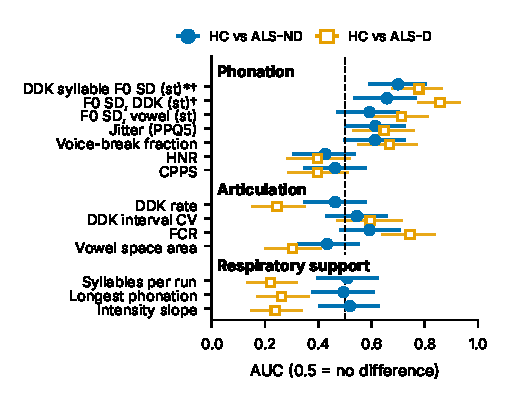
\includegraphics[width=\columnwidth]{fig1_forest}
\caption{Selected main measures (all \nFeat{} in the repository), HC vs.\ ALS-ND (filled) and HC vs.\ ALS-D (hollow): AUC with 95\% bootstrap CI. $^*$ $q<0.05$; $^\dagger$ $q_{\rm adj}<0.05$ (rank-based age/sex adjustment), HC vs.\ ALS-ND.}
\label{fig:forest}
\end{figure}

\textbf{Is the marker real?} On the same 10\,ms track, the syllable $F_0$ SD splits into an octave-folded spread (AUC \rFoldAUC{} [\rFoldLo, \rFoldHi], $p=\rFoldP$) and octave-level events (share \rOctAUC{} [\rOctLo, \rOctHi], $p\,\rOctP$; median \rOctMedHC\% in HC vs.\ \rOctMedND\%); the exploratory 2\,ms versions agree (\eMacroAUC, $q=\eMacroQ$; \eOctDAUC, $q=\eOctDQ$). Of the \shrDown{} nuclei flagged more than 6\,st \emph{below} the median (the \shrUp{} above it are not tested), \shrDownGenuine{} (\shrDownPct\%) exceed the SHR criterion, against \shrCtrlAbove{} of \shrCtrlN{} unflagged nuclei (\shrCtrlFP\%), so most octave-down events carry real subharmonic energy---period doubling, the subharmonic regime of an unstable vocal-fold oscillator~\cite{herzel1994nonlinear}, or a creak-like register---rather than tracking errors (Fig.~\ref{fig:example}). That control rate is not purely false positives: unflagged nuclei are subharmonic more often in ALS-ND (pooled \rUnflRateND\% vs.\ \rUnflRateHC\%; per-speaker median \rUnflMedND\% vs.\ \rUnflMedHC\%, AUC \rUnflAUC, $p=\rUnflP$). Measured at every nucleus at half its octave-folded $F_0$, the share of subharmonic nuclei also separates the groups (AUC \rSubhAUC{} [\rSubhLo, \rSubhHi], $p=\rSubhP$; median \rSubhMedHC\% vs.\ \rSubhMedND\%); with half the speaker's median as the only pitch input it is borderline (\rSubhMedAUC, $p=\rSubhMedP$).

\textbf{End of run and pitch tracker.} Octave events are commoner at the end of runs, as end-of-breath creak would be: \rPosHCLast\% of the \rPosHCN{} control events and \rPosNDLast\% of the \rPosNDN{} ALS-ND events fall in the last third of a run, which holds a third of the nuclei (\rSingleRun\% of recordings are a single run). The contrast does not depend on them: without the last \rDropLast{} syllables of each run the octave share gives \rOctTrimAUC{} and the syllable $F_0$ SD \rSdTrimAUC{} (folded \rFoldTrimAUC), and the first two thirds of runs alone give \rOctEarlyAUC. The tracker matters more. Praat's autocorrelation method and a 75\,Hz floor leave the unfolded SD at \trkMin--\trkMax{} and the folded SD at \trkFoldMin--\trkFoldMax. With REAPER, which shares no code with Praat, the unfolded SD weakens (\trkRpr, $p=\trkRprP$), the octave share is lost (\trkOctRpr, $p=\trkOctRprP$; per-speaker agreement with Praat $\rho=\trkOctRprSame$) and so is the spectral subharmonic share (\rSubhRprAUC, $p=\rSubhRprP$), whereas the folded SD is stable (\trkFoldRpr, $p=\trkFoldRprP$; $\rho=\trkFoldRprSame$). In place of the Praat marker in the \nFeat-measure family none would pass correction ($q=\trkRprQ$ unfolded and \trkFoldRprQ{} folded with REAPER, \trkFoldCcQ{} folded with Praat). DDK level, SNR, rate, syllable count and mean $F_0$ do not differ between groups (AUC \covRateAUC--\covLevelAUC); rank-based residualisation on age, sex, SNR, level, rate and syllable count leaves AUC \covAdjAUC{} ($p\covAdjP$). Within a session the marker is moderately consistent across syllable types (ICC(2,1) \iccAll; split-half Spearman--Brown \sbMin--\sbMax).

\textbf{Which task, which features.} Per-task models on our measures reach at most \tkaAUC{} (/ka/; vowels \toAUC--\tiAUC, all tasks \tallAUC), and the syllable $F_0$ SD alone \tddkoneAUC{} [\tddkoneLo, \tddkoneHi] averaged over the syllable tasks (chosen on these data, hence optimistic). The generic set reaches \abAllAll{} [\abAllAllLo, \abAllAllHi] with all tasks and \gSingleMin--\gSingleMax{} with single tasks (the best, \gBestTask, is one of eight post-hoc choices); adding MFCC statistics lowers it (\gAllMAUC). The ablation (Table~\ref{tab:ablation}) shows a crossover: on the syllable tasks the four $F_0$ functionals carry the signal (\abFzDdkMin--\abFzDdkMax) and the other eight descriptors are at chance (\abNfDdkMin--\abNfDdkMax); on vowels the reverse holds (\abNfVowMin--\abNfVowMax{} vs.\ \abFzVowMin--\abFzVowMax). The intensity/duration/voicing block (\abIdvAll{} with all tasks) is driven by mean intensity (vowels AUC \idvIntVAUC, $p=\idvIntVP$; patients tend to be louder, median \idvIntVMedND{} vs.\ \idvIntVMedHC\,dB; without intensity the block falls to \idvNoInt) and by voiced fraction (DDK \idvVoicedDAUC; without it \idvNoVoiced), not by duration (\idvDurVAUC, \idvDurDAUC): an uncalibrated recording level and the voicing of the syllable train, i.e.\ task execution and possibly voice onset, rather than respiratory support.

\begin{table}[t]
\centering\scriptsize
\caption{Ablation of the generic set, HC vs.\ ALS-ND: cross-validated AUC of one descriptor block from single syllable tasks or vowels (range over tasks) or from all tasks (vowel and DDK means), and the age/sex floor. $^\ddagger$Median and 2.5--97.5\% range of the permutation null.}
\label{tab:ablation}
\setlength{\tabcolsep}{2pt}
\begin{tabular}{@{}lccc@{}}
\toprule
Block & /pa/, /ta/, /ka/ & 5 vowels & All tasks [95\% CI] \\
\midrule
$F_0$ functionals (4) & 0.64--0.69 & 0.42--0.60 & 0.68 [0.57, 0.78] \\
Voice quality (3) & 0.50--0.52 & 0.53--0.67 & 0.57 [0.45, 0.68] \\
Intens., dur., voicing (5) & 0.51--0.57 & 0.56--0.61 & 0.64 [0.53, 0.75] \\
All but $F_0$ (8) & 0.50--0.57 & 0.63--0.74 & 0.67 [0.56, 0.77] \\
All 12 & 0.60--0.66 & 0.63--0.73 & 0.67 [0.57, 0.78] \\
\midrule
Age + sex only & -- & -- & 0.47 [0.35, 0.57] \\
Permutation null, all 12 & -- & -- & 0.49 [0.32, 0.62]$^\ddagger$ \\
\bottomrule
\end{tabular}

\end{table}

\textbf{Time scale and stage of phonation.} Fig.~\ref{fig:timescale}: in sustained vowels the extra $F_0$ modulation is not confined to the 4--8\,Hz tremor band (\eTremorAUC); after adjustment the slow-wander (0.25--1\,Hz, \eWanderAUC; adjusted \eWanderAdj) and flutter bands (8--15\,Hz, \eFlutterAUC) differ, the 1--4\,Hz band falls short (\eSlowAUC, $q_{\rm adj}=\eSlowQadj$), and the band \emph{shares} are unchanged (\eWanderRelAUC, \eTremorRelAUC): the modulation spectrum is scaled up, not reshaped. Slow wander of vowel intensity also differs after adjustment (\eIntWanderAUC; adjusted \eIntWanderAdj). In the DDK task the variation sits between syllables, not within them: within-nucleus SD at chance (\eMicroAUC), detrending does not reduce the group difference (\eMacroDetrAUC), lag-1 autocorrelation unchanged (\eLagAUC). The SD of $F_0$ at voicing onset (unfolded, so partly counting octave events; \eOnsetAUC; adjusted \eOnsetAdj, $q_{\rm adj}=\eOnsetQadj$) and the burst-to-voicing delay (\eVotAUC, $q=\eVotQ$) differ; the amplitude rise time does not (\eRiseAUC) until dysarthria (\eRiseDAUC).

\begin{figure}[t]
\centering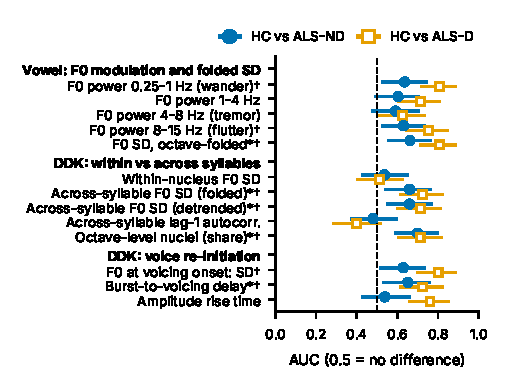
\includegraphics[width=\columnwidth]{fig4_timescale}
\caption{Time scale and stage of the laryngeal instability: AUC (95\% CI), HC vs.\ ALS-ND (filled) and HC vs.\ ALS-D (hollow). $^*$ $q<0.05$; $^\dagger$ $q_{\rm adj}<0.05$, HC vs.\ ALS-ND, one family of \nExt{} measures.}
\label{fig:timescale}
\end{figure}

\begin{table}[t]
\centering\scriptsize
\caption{Spearman $\rho$ with clinical scores in the 102 patients ($n$ = 96--102 per cell); bold: $q<0.05$. Bulbar = ALSFRS-R speech + salivation + swallowing. PUMNS: higher = worse; other scores: higher = better.}
\label{tab:clin}
\setlength{\tabcolsep}{3.5pt}
\begin{tabular}{@{}lccccc@{}}
\toprule
Measure & PUMNS & MRC & Bulbar & FVC & Dyspnea \\
\midrule
DDK syllable $F_0$ SD & -0.04 & -0.14 & -0.13 & -0.22 & \textbf{-0.27} \\
$F_0$ SD, DDK & 0.12 & \textbf{-0.33} & \textbf{-0.36} & \textbf{-0.33} & \textbf{-0.33} \\
Jitter (PPQ5) & -0.08 & -0.22 & -0.15 & -0.18 & \textbf{-0.27} \\
DDK rate & \textbf{-0.33} & \textbf{0.46} & \textbf{0.50} & \textbf{0.33} & \textbf{0.23} \\
FCR & \textbf{0.27} & \textbf{-0.31} & \textbf{-0.36} & \textbf{-0.25} & -0.16 \\
Syllables per run & \textbf{-0.39} & \textbf{0.68} & \textbf{0.67} & \textbf{0.61} & \textbf{0.43} \\
Longest phonation & -0.25 & \textbf{0.57} & \textbf{0.53} & \textbf{0.51} & \textbf{0.39} \\
Intensity slope & \textbf{-0.31} & \textbf{0.58} & \textbf{0.57} & \textbf{0.41} & \textbf{0.41} \\
\bottomrule
\end{tabular}

\end{table}

\textbf{Clinical anchoring, pathway, progression.} Within the 102 patients (Table~\ref{tab:clin}) the respiratory and articulatory measures track severity: syllables per run correlates with MRC head strength ($\rho=\mrcSylRho$), the ALSFRS-R bulbar sum (\bulSylRho), FVC\,\% (\fvcSylRho; cf.~\cite{stegmann2021fvc,tabor2023mpt}) and PUMNS bulbar burden ($\pumnsSylRho$), all $q\leq0.002$; these severity measures are at chance in normal-rated speech, while the normal-rated markers are weak severity markers (syllable $F_0$ SD: dyspnea item only, $\rho=\ndallDyspRho$). In partial correlations the measures align with head-muscle strength (MRC, a lower-motor-neuron-weighted proxy; controlling PUMNS and age, \pNLmnSig{} of \pN{} measures at $q<0.05$, e.g.\ syllables per run \pSylLmn, but not the syllable $F_0$ SD, $\pSylFLmn$) and none with PUMNS once MRC and age are controlled ($q\geq\pUmnMinQ$). Within ALS-ND no measure is associated with progression rate ($q\geq\gNdMinQ$); across all patients faster progression goes with a steeper intensity decline ($\rho=\gIntRho$, $q<0.001$).

\section{Discussion}
\label{sec:discussion}
\textbf{What differs, and what it may mean.} In spinal-onset patients rated as speaking normally, the clearest difference is in laryngeal control: the spread of $F_0$ between syllable re-onsets and more frequent subharmonic re-onsets, not confined to the end of runs, with HNR and CPPS at chance; vowels carry a separate signal from voice quality and mean level, the latter possibly task execution. $F_0$ variability itself is visible in the released VOC-ALS values~\cite{dubbioso2024vocals}; we show what it consists of and how far it depends on the tracker. Read through the motor pathway, each re-onset requires the laryngeal motoneurons of the nucleus ambiguus to re-establish vocal-fold tension and adduction within tens of milliseconds; a pool losing motor units could set that target less reproducibly (between-syllable spread, onset $F_0$ deviation) and enter the subharmonic regime more often~\cite{herzel1994nonlinear}, while holding a steady state once reached (within-nucleus SD at chance, intact amplitude rise). This is a hypothesis: the marker relates to neither MRC nor PUMNS, which score other muscles or reflexes, and subglottal pressure at onset (suggested by the dyspnea correlation) and task execution remain alternatives, although adjusting for level, rate and syllable count did not weaken the effect. The articulatory null is limited to our tasks: the speaking-rate and precision changes of Stegmann et al.~\cite{stegmann2020early} were found in read sentences, which a self-paced DDK and sustained vowels do not probe, and the phonatory--articulatory difference itself is uncertain.

\textbf{Implications for measurement.} Nucleus-level $F_0$ in semitones with octave events counted apart from the folded spread, spectral checks of subharmonics, and permutation nulls rather than 0.5 all matter. As the unfolded spread, the octave share and even the spectral share (which inherits the tracker's within-octave $F_0$) weaken with an independent tracker, the tracker must be fixed and reported and cross-tracker agreement belongs in validation. For home monitoring, an ICC of \iccAll{} means several recordings per time point, and test--retest reliability is still to be measured.

\textbf{Limitations.} Cross-sectional, one site, language and device; the reference standard is one perceptual item; ALS-ND is spinal-onset only and most have some bulbar finding (only \sensDN{} have normal bulbar items, head strength and PUMNS, a tier whose CI includes 0.5); the DDK was self-paced, which weakens respiratory proxies and the rate measure; subharmonic events were validated spectrally, not perceptually; the measures were chosen on these data, so AUCs are optimistic, and effects of 0.6--0.7 indicate group-level change, not screening. Longitudinal recordings would test whether the laryngeal change precedes bulbar decline.

\section{Conclusion}
\label{sec:conclusion}
In VOC-ALS, ALS patients with normal-rated speech differ from controls in the spread of $F_0$ across successive syllable re-onsets---a between-syllable instability, not confined to the end of runs---and in more subharmonic re-onsets. Both depend on the pitch tracker; the octave-folded spread is stable across trackers but only nominal, and the advantage over articulatory measures is not established.

\bibliographystyle{IEEEbib}
\bibliography{refs}
\end{document}
